\section{Results}
\label{sec:results}

\subsection{Phase 1: zero-shot baselines}
\label{sec:res-phase1}

Phase~1 measured the zero-shot performance of the four lightweight VLMs on the
three medical VQA datasets, answering RQ1. Evaluation used seed 42 on the full
test split of each dataset (PathVQA 6,719 / SLAKE 1,061 / VQA-RAD 451 items).
The per-condition results are given in Table~\ref{tab:phase1}.

\begin{table}[t]
\centering
\caption{Zero-shot baseline results (model $\times$ dataset). Open items are
scored by BERTScore (roberta-large backbone, threshold method) and closed items
by exact string match against the gold answer; Overall Acc is computed over
closed and open items combined.}
\label{tab:phase1}
\small
\begin{tabular}{@{}llrrrrrr@{}}
\toprule
Model & Dataset & Closed & Open & Overall & BERTScore F1 & Time (ms) & VRAM (MB) \\
\midrule
Gemma4-E2B    & PathVQA & 0.1633 & 0.0477 & 0.1055 & 0.8069 & 892.6 & 13,932.7 \\
Gemma4-E2B    & SLAKE   & 0.6394 & 0.4178 & 0.4920 & 0.8679 & 689.8 & 13,927.3 \\
Gemma4-E2B    & VQA-RAD & 0.4502 & 0.3100 & 0.3880 & 0.8373 & 721.5 & 13,929.1 \\
Qwen2.5-VL-3B & PathVQA & 0.6130 & 0.0354 & 0.3245 & 0.8613 & 483.4 & 7,581.3 \\
Qwen2.5-VL-3B & SLAKE   & 0.7465 & 0.4632 & 0.5580 & 0.9359 & 254.8 & 7,561.9 \\
Qwen2.5-VL-3B & VQA-RAD & 0.6614 & 0.2800 & 0.4922 & 0.8886 & 310.6 & 7,580.5 \\
Qwen3-VL-2B   & PathVQA & 0.6336 & 0.0605 & 0.3472 & 0.8487 & 419.1 & 4,527.3 \\
Qwen3-VL-2B   & SLAKE   & 0.7915 & 0.4575 & 0.5693 & 0.9081 & 344.9 & 4,412.9 \\
Qwen3-VL-2B   & VQA-RAD & 0.7211 & 0.2250 & 0.5011 & 0.8894 & 245.7 & 4,428.5 \\
SmolVLM2-2.2B & PathVQA & 0.5892 & 0.0274 & 0.3085 & 0.8557 & 666.0 & 6,021.3 \\
SmolVLM2-2.2B & SLAKE   & 0.6648 & 0.3598 & 0.4618 & 0.9130 & 774.7 & 5,991.2 \\
SmolVLM2-2.2B & VQA-RAD & 0.6574 & 0.3150 & 0.5055 & 0.9029 & 756.7 & 5,996.2 \\
\bottomrule
\end{tabular}
\end{table}

\subsubsection{Differences across models}

On pooled accuracy over all three datasets ($n = 8{,}231$ items), the ranking is
Qwen3-VL-2B 0.3843 (95\% CI [0.3740, 0.3947]), Qwen2.5-VL-3B 0.3637 ([0.3533,
0.3740]), SmolVLM2-2.2B 0.3391 ([0.3289, 0.3495]), and Gemma4-E2B 0.1708
([0.1627, 0.1790]). Cochran's $Q$ test shows that the correctness patterns of
the four models differ significantly on a pooled basis ($Q = 1904.28$, $df = 3$,
$p < .001$); tested on each dataset individually, all three are also significant
(PathVQA $Q = 2067.08$, SLAKE $Q = 71.34$, VQA-RAD $Q = 27.18$; all $p < .001$).

In pairwise McNemar post-hoc tests with Bonferroni correction, Gemma4-E2B
performed significantly worse than all three other models on the pooled basis and
on PathVQA and VQA-RAD individually (all such comparisons $p(\mathrm{adj}) <
.005$). SLAKE is an exception: the difference between Gemma4-E2B and
SmolVLM2-2.2B is not significant there (0.492 vs.\ 0.462, $p(\mathrm{adj}) =
0.326$), Gemma4-E2B performing relatively better on SLAKE than on the other two
datasets. Among the three leading models, all three pairs differ significantly on
the pooled basis ($p(\mathrm{adj}) < .001$), yet on SLAKE and VQA-RAD
individually the difference between Qwen2.5-VL-3B and Qwen3-VL-2B is not
significant ($p(\mathrm{adj}) = 1$ in both cases). Qwen3-VL-2B is thus the best
model on pooled accuracy, but it is close enough to Qwen2.5-VL-3B that the two
are not statistically separable on some datasets.

\paragraph{Contamination robustness.}
Samples suspected of pretraining exposure were identified by the Min-$K$\%
Probability analysis ($K = 20\%$, outliers in the top 5\% within each dataset:
1,020 for PathVQA, 233 for SLAKE, 73 for VQA-RAD, taken as the union across the
four models), removed, and the same tests re-run. Cochran's $Q$ remained
significant on all three datasets, and the pooled model ranking and the best
model (Qwen3-VL-2B) were preserved (original 0.3843 $\rightarrow$ reduced set
0.3037: absolute accuracy falls but the ranking is unchanged). The full ranking
is preserved position for position: Qwen3-VL-2B $>$ Qwen2.5-VL-3B $>$
SmolVLM2-2.2B $>$ Gemma4-E2B holds both before removal (0.3843, 0.3637, 0.3391,
0.1708) and after (0.3037, 0.2765, 0.2660, 0.1076). The conclusions of this
subsection are therefore robust to potential data contamination, in the sense
that the ordering survives; the absolute drop of roughly eight percentage points
is itself substantial and is discussed as a limitation in
Section~\ref{sec:discussion}.

\subsubsection{Dataset difficulty}

The difficulty ordering of the three datasets is independent of the model.
Comparing the mean Overall Acc of the four models by dataset gives PathVQA (mean
0.271) $<$ VQA-RAD (mean 0.472) $<$ SLAKE (mean 0.520), so PathVQA is markedly
harder than the other two. The gap is concentrated in open-ended items: on all
three datasets open accuracy (0.03--0.46) is far below closed accuracy
(0.45--0.79), but the drop is most severe on PathVQA, whose open accuracy is
0.027--0.061 across all models --- more than an order of magnitude below SLAKE
(0.360--0.463) and VQA-RAD (0.225--0.315). PathVQA contains a high proportion of
items requiring free-form description of detailed findings in pathology tissue
images, so generative open-ended responses are interpreted as being harder than
on SLAKE and VQA-RAD, which contain relatively more multiple-choice-type items.

Response time and VRAM scale with model size, and differences across datasets are
negligible (VRAM variation across datasets within the same model is $< 1\%$).
Response time does vary somewhat by model according to item characteristics such
as the length of description required --- Gemma4-E2B takes 892.6\,ms on PathVQA,
longer than on SLAKE or VQA-RAD.

\subsubsection{Error types}

For the WCA analysis, PathVQA items (seed 42) were classified into the seven
clinical question types and accuracy computed per type; the full table is
deferred to Appendix~\ref{app:tables} (Table~\ref{tab:apptypes}). As noted in
Section~\ref{sec:stats}, the weights are a provisional scale without
clinical-literature validation and are used only to identify reference error
patterns.

The most striking pattern is that all four models score exactly 0.0000 on the
diagnosis and temporal types. Although diagnosis carries the highest WCA weight
(1.0) and is clinically the most important type, the models in their zero-shot
state were entirely unable to derive a diagnostic name from pathological
findings. The description type (free-form narration) also remains at 0.02--0.04
accuracy despite having the largest sample count (2,729 items, 41\% of the
total), and is confirmed as the principal factor depressing overall PathVQA
accuracy. Conversely the yes\_no type shows relatively high accuracy (0.6336 for
Qwen3-VL-2B, for example), and the ranking across models largely matches the
pooled ranking above; Gemma4-E2B nevertheless lags far behind the other three
even on yes\_no (0.1633 versus 0.59--0.63), confirming that its inferiority is
not confined to particular types. Zero-shot lightweight VLMs can thus cope to
some degree with binary discrimination, but are effectively unable to handle
clinically important open-ended tasks such as deriving a diagnosis or generating
free-form descriptions of findings.

\subsection{Phase 2: QLoRA fine-tuning}
\label{sec:res-phase2}

Phase~2 fine-tuned each of the four models on each of the three datasets with
QLoRA (rank $=64$, alpha $=128$, target $=$ all-linear, ceiling
\texttt{max\_steps}~$=500$) and verified RQ2. In addition to the 36 main
conditions (4 models $\times$ 3 datasets $\times$ 3 seeds), 39 further
conditions were run under fixed Qwen3-VL-2B and PathVQA settings for Ablations A,
B, and C, giving 75 conditions in total.

\subsubsection{Base versus fine-tuned performance}

Per-model performance before and after fine-tuning, with the paired tests, is
given in Table~\ref{tab:phase2ft}.

\begin{table}[t]
\centering
\caption{Fine-tuning effect by model (paired, $n = 9 = 3$ datasets $\times$ 3
seeds).}
\label{tab:phase2ft}
\small
\begin{tabular}{@{}lrrrlll@{}}
\toprule
Model & Base Acc & FT Acc & Cohen's $d$ & $d$ 95\% CI (BCa) & paired $t$ $p$ & Wilcoxon $p$ \\
\midrule
Qwen2.5-VL-3B & 0.4582 & 0.5749 & $+2.646$ & [1.953, 4.723]   & $< .001$ & .0039 \\
Qwen3-VL-2B   & 0.4725 & 0.5845 & $+1.620$ & [0.932, 3.153]   & .0013    & .0039 \\
SmolVLM2-2.2B & 0.4253 & 0.4036 & $-2.284$ & [$-3.160$, $-1.552$] & $< .001$ & .0039 \\
Gemma4-E2B    & 0.3285 & 0.2288 & $-0.652$ & [$-1.599$, 0.032]    & .0864 (n.s.) & .1289 (n.s.) \\
\bottomrule
\end{tabular}
\end{table}

The effect of fine-tuning is heterogeneous across models. Qwen2.5-VL-3B and
Qwen3-VL-2B improved significantly ($p < .01$, large effect size), whereas
SmolVLM2-2.2B significantly deteriorated, and Gemma4-E2B moved in a negative
direction without reaching statistical significance. All three tests reached
consistent conclusions for each model, supporting the robustness of the result.

A mixed-effects model estimated by pooling the four models without distinguishing
them (\texttt{accuracy $\sim$ condition $+$ dataset}, group $=$ seed) found no
significant fixed effect (coefficient $= 0.0268$, $p = .3629$, ICC(seed) $= 0.0$,
$n = 72$). This is not a computational error but a consequence of heterogeneous
effects across models cancelling in the pooled mean. The per-model triple
verification is therefore taken as the primary evidence for RQ2, and the pooled
result is cited only as supporting explanation that the overall effect without
distinguishing models is not significant because of heterogeneity.

\subsubsection{Ablations A, B, and C}

The three ablations, each with PathVQA and Qwen3-VL-2B held fixed and each
reported as the mean of 3 seeds, are consolidated in Table~\ref{tab:ablations}.

\begin{table}[t]
\centering
\caption{Ablations A (data ratio), B (LoRA rank), and C (target-module scope).
Qwen3-VL-2B, PathVQA, mean of 3 seeds.}
\label{tab:ablations}
\small
\begin{tabular}{@{}lrr@{\hspace{2em}}lrr@{\hspace{2em}}lrr@{}}
\toprule
\multicolumn{3}{c}{A: data ratio} & \multicolumn{3}{c}{B: LoRA rank} & \multicolumn{3}{c}{C: target modules} \\
\cmidrule(r){1-3}\cmidrule(r){4-6}\cmidrule(l){7-9}
ratio & samples & Acc & rank & VRAM (MB) & Acc & scope & trainable & Acc \\
\midrule
0.05 & 982    & 0.4150 & 4  & 3,870.6 & 0.4733 & minimal & 0.21\% & 0.5015 \\
0.10 & 1,965  & 0.4309 & 8  & 3,875.2 & 0.4907 & medium  & 0.43\% & 0.5155 \\
0.25 & 4,913  & 0.4357 & 16 & 3,884.4 & 0.5020 & full    & 1.55\% & 0.5400 \\
0.50 & 9,827  & 0.4628 & 32 & 3,902.8 & 0.5172 & & & \\
1.00 & 19,654 & 0.5019 & 64 & 3,918.8 & 0.5210 & & & \\
\bottomrule
\end{tabular}
\end{table}

Accuracy increases monotonically with the training-data ratio, with no sign of
reaching a ceiling over the interval from 0.05 to 1.0; within the experimental
range, using the full dataset (ratio $=1.0$) is optimal. Performance also
increases monotonically with LoRA rank, though the gain flattens between 32 and
64 ($+0.0038$ from 32 to 64 versus $+0.0152$ from 16 to 32), while the VRAM
increase across the whole range from rank 4 to 64 is a negligible 1.3\%
(3,870.6 $\rightarrow$ 3,918.8\,MB); since the performance gain relative to VRAM
cost remains positive, rank $=64$ was adopted. Performance likewise increases
monotonically as the target-module scope widens, with full (all-linear) giving
the best of the three settings, and it was adopted as the default configuration
of the Phase~2 main experiment. These three axes were each verified independently
with the other two held fixed; the combination applying all three optima
simultaneously was not itself separately verified.

We note one measurement artefact identified in the Phase~2 logs. The
\texttt{train\_time\_min} column of the Phase~2 summary is unusually large for
seed 42 alone under identical conditions (at ratio $=1.0$, seed 42 is 369.6
minutes versus about 28 minutes for seeds 123 and 456). Direct comparison against
each condition's training record showed that \texttt{train\_runtime\_sec},
measured internally by the Trainer, was consistently normal at 27--29 minutes
across all seeds; the defect lies only in the wall-clock measurement of the
wrapping script and appears in the condition that first creates the preprocessing
cache for a (model, dataset) combination (for example, Qwen2.5-VL-3B on PathVQA
seed 42 at 395.4 minutes versus 44.9 minutes actual). Accuracy and loss are
unaffected, and the accuracy-based conclusions are unchanged.

\subsubsection{Catastrophic forgetting}

Both measurements of forgetting are given in Table~\ref{tab:cf}: (A) the change
in general capability on a VQAv2 validation subset (2,000 samples), and (B) the
rate of performance change when evaluated on a dataset other than the training
domain.

\begin{table}[t]
\centering
\caption{Catastrophic forgetting. (A) VQAv2 performance degradation rate, $n = 9$
(3 datasets $\times$ 3 seeds). (B) Cross-dataset performance change rate,
$n = 18$ (2 eval sets $\times$ 3 training sets $\times$ 3 seeds).}
\label{tab:cf}
\small
\begin{tabular}{@{}lrrl@{\hspace{2em}}rrr@{}}
\toprule
& \multicolumn{3}{c}{(A) VQAv2 degradation} & \multicolumn{3}{c}{(B) Cross-dataset change} \\
\cmidrule(r){2-4}\cmidrule(l){5-7}
Model & Mean (\%) & SD & Range & Mean (\%) & SD & Share positive \\
\midrule
Gemma4-E2B    & 51.50 & 4.74 & 43.50 -- 57.49 & $+73.94$ & 79.97 & 15/18 \\
Qwen3-VL-2B   & 7.23  & 3.11 & 3.29 -- 10.47  & $-9.46$  & 9.23  & 3/18 \\
Qwen2.5-VL-3B & 4.42  & 3.60 & $-0.34$ -- 8.30 & $+0.38$ & 4.98  & 9/18 \\
SmolVLM2-2.2B & 0.49  & 0.29 & 0.15 -- 0.96   & $-31.53$ & 17.49 & 0/18 \\
\bottomrule
\end{tabular}
\end{table}

General-capability loss diverges sharply across models. Gemma4-E2B loses on
average 51.5\% of its VQAv2 performance after fine-tuning, exhibiting clear
catastrophic forgetting, whereas SmolVLM2-2.2B shows essentially no degradation
(mean 0.49\%). This ordering runs opposite to the ranking of domain improvement
above: the Qwen family, which gained most in the domain, gives up some general
capability (4--7\%), Gemma4-E2B suffers a double loss (neither significant domain
improvement nor retention of general capability), and SmolVLM2-2.2B preserves
general capability but significantly deteriorates in the domain. This is an
observed pattern; no causal relationship was verified.

Because PathVQA (pathology tissue) and SLAKE/VQA-RAD (radiological images) differ
in image domain itself, panel (B) is interpreted as a domain-generalization gap
rather than catastrophic forgetting in the strict sense. SmolVLM2-2.2B shows a
clear fall in performance on other datasets the more it specializes on one (mean
$-31.5\%$, negative in all 18 conditions), whereas Gemma4-E2B rises substantially
on average ($+73.9\%$) with extreme variability (SD 79.97, ranging from $-8.06\%$
to $+205.56\%$). This large positive mean may be a floor effect arising from the
low zero-shot baseline identified in Section~\ref{sec:res-phase1} (about 0.10 on
PathVQA in particular): when base accuracy is very low, relative change rates are
easily exaggerated in either direction.

\subsection{Phase 3: autonomous hyperparameter optimization}
\label{sec:res-phase3}

Phase~3 fixed Qwen3-VL-2B --- the best performer in Phase~2 --- on PathVQA and
compared the four search strategies under identical conditions, answering RQ3.
Training volume was controlled at \texttt{max\_steps}~$=200$ for all trials, and
the execution scale of the four-strategy comparison was 610 trials in total; with
the 200-trial configuration-consistency re-experiment reported in
Section~\ref{sec:res-v2}, Phase~3 comprises 810 trials overall. As described in
Section~\ref{sec:phase3}, statistical testing is performed only at the run level:
the unit of testing is the 10 per-repeat best \texttt{val\_accuracy} values
obtained from the 10 independent repeats of each strategy (for Manual, which has
one trial per repeat, that value is itself the run-level value), and trial-level
data are used only for describing the search process.

\subsubsection{Run-level comparison of strategies}
\label{sec:res-runlevel}

Run-level performance is given in the upper panel of Table~\ref{tab:phase3run}. A
run-level value is the highest \texttt{val\_accuracy} among the completed trials
of each independent repeat; failed trials (status $\neq$ completed) are excluded
from aggregation. Under the Manual strategy there are records of 10 failures
followed by retries in repeats 6--9, but every repeat ultimately completed one
trial successfully, so the run-level sample size of 10 is preserved.

\begin{table}[t]
\centering
\caption{Run-level performance by HPO strategy ($n = 10$ per condition, the
per-repeat best \texttt{val\_accuracy} over 10 independent repeats). The
Autoresearch-v2 condition (Section~\ref{sec:res-v2}) differs from the original in
prompt and constraints and is reported separately rather than folded into the
four-strategy same-condition comparison.}
\label{tab:phase3run}
\small
\begin{tabular}{@{}lrl@{}}
\toprule
Strategy & Mean \texttt{val\_accuracy} & 95\% CI (bootstrap) \\
\midrule
\multicolumn{3}{@{}l}{\emph{Four-strategy comparison}} \\
Optuna (TPE)       & 0.4490 & [0.4368, 0.4594] \\
Random Search      & 0.4186 & [0.4106, 0.4274] \\
Autoresearch (LLM) & 0.4184 & [0.4064, 0.4328] \\
Manual             & 0.3776 & [0.3760, 0.3794] \\
\midrule
\multicolumn{3}{@{}l}{\emph{Reported separately}} \\
Autoresearch-v2    & 0.4292 & [0.4124, 0.4478] \\
\bottomrule
\end{tabular}
\end{table}

The difference in run-level performance among the four strategies is
statistically significant under the Kruskal--Wallis test ($H = 27.92$, $df = 3$,
$p < .001$). The Mann--Whitney $U$ test for the comparison central to RQ3,
Autoresearch versus Optuna, is significant at $U = 16.00$, $p = .0112$,
rank-biserial $r = -0.68$. Under the sign convention adopted here, $r > 0$ means
the first sample (Autoresearch) is stochastically superior to the second
(Optuna), so a negative $r$ means Optuna is significantly superior to
Autoresearch. The direction is confirmed independently of the test by the
confidence intervals: the lower bound of Optuna's interval (0.4368) exceeds the
upper bound of Autoresearch's (0.4328), so the two intervals do not overlap. By
contrast, Autoresearch (0.4184) and Random Search (0.4186) have practically
identical means with largely overlapping intervals and are not statistically
distinguishable.

The ordering among strategies under these experimental conditions is therefore
Optuna $>$ (Random $\approx$ Autoresearch) $>$ Manual. The LLM agent's autonomous
search fell significantly short of established Bayesian optimization and showed
no advantage even over random search. All three automated strategies including
Autoresearch nevertheless exceeded the researcher's manual configuration
(0.3776), confirming the validity of automated hyperparameter search as such.

\subsubsection{Hyperparameters found by each strategy}

The configuration of the best-performing trial reached by each strategy is given
in Table~\ref{tab:phase3best}. This table describes a single best configuration
per strategy; the sample size is one, and it is not used as evidence for the
relative merit of the strategies, which is judged by the run-level tests above.

\begin{table}[t]
\centering
\caption{Hyperparameter configuration of the best-performing trial per strategy.
The closed and open columns are the \texttt{val\_closed\_acc} and
\texttt{val\_open\_acc} of that trial.}
\label{tab:phase3best}
\footnotesize
\begin{tabular}{@{}lrrrrrrrlrrr@{}}
\toprule
Strategy & rank & alpha & lr & batch & g.acc & warmup & w.decay & targets & val\_acc & closed & open \\
\midrule
Manual       & 16 & 32  & 2.00e-4 & 1 & 8  & 0.030 & 0.010 & minimal & 0.3840 & 0.7213 & 0.0625 \\
Random       & 64 & 256 & 2.08e-4 & 2 & 16 & 0.072 & 0.013 & full    & 0.4440 & 0.7951 & 0.1094 \\
Optuna       & 32 & 128 & 4.91e-4 & 4 & 16 & 0.089 & 0.054 & full    & 0.4700 & 0.8115 & 0.1445 \\
Autoresearch & 64 & 256 & 2.00e-4 & 4 & 16 & 0.050 & 0.010 & full    & 0.4640 & 0.7992 & 0.1445 \\
\bottomrule
\end{tabular}
\end{table}

In all four strategies the gap between closed accuracy (0.72--0.81) and open
accuracy (0.06--0.14) persists. The overall accuracy gain achieved by search
(Manual 0.3840 $\rightarrow$ Optuna 0.4700) arose mainly on closed items, while
open accuracy remains at 0.1445 even under the best configuration, so the
weakness in open-ended responses observed in Phase~1 was not resolved by
hyperparameter optimization.

The three strategies that explored the search space freely (Random, Optuna,
Autoresearch) all converged on \texttt{lora\_targets=full} (all-linear) with rank
in the 32--64 region. This coincides independently with the finding of Ablations
B and C that rank $=64$ and target $=$ all-linear are optimal; two different
experimental designs --- fixed-axis ablation and free search --- pointing to the
same region reinforces the Phase~2 conclusion. The best-performing Optuna
configuration, meanwhile, combined rank $=32$ with a relatively high learning
rate (4.91e-4) and weight decay (0.054), a region the other strategies did not
reach.

\subsubsection{Search trajectory (trial level, descriptive only)}
\label{sec:res-traj}

Table~\ref{tab:phase3trial} summarizes the search process at the trial level.

\begin{table}[t]
\centering
\caption{Trial-level description of the search process. The left panel gives the
trial at which the best performance was reached over 10 repeats; the right panel
gives the distribution over all 200 trials per strategy. Descriptive statistics
only.}
\label{tab:phase3trial}
\small
\begin{tabular}{@{}lrrl@{\hspace{2em}}rrr@{}}
\toprule
& \multicolumn{3}{c}{Trial of best (10 repeats)} & \multicolumn{3}{c}{All trials} \\
\cmidrule(r){2-4}\cmidrule(l){5-7}
Strategy & Final best (med.) & Trial (med.) & IQR & Mean & SD & Train time (min) \\
\midrule
Manual        & 0.3770 & 1.0  & ---           & 0.3776 & 0.0031 & 228.3 \\
Random Search & 0.4150 & 15.0 & [12.2, 17.0]  & 0.3672 & 0.0321 & 5,078.6 \\
Optuna (TPE)  & 0.4550 & 15.0 & [13.5, 18.0]  & 0.3905 & 0.0374 & 5,967.3 \\
Autoresearch  & 0.4060 & 17.5 & [11.5, 20.0]  & 0.3980 & 0.0145 & 5,450.0 \\
\bottomrule
\end{tabular}
\end{table}

Autoresearch reaches its best performance latest, with a median trial of 17.5,
and the upper bound of its IQR touches 20.0, the ceiling of the search budget.
Nearly half of the runs were therefore still improving at the point the budget was
exhausted, suggesting that a budget of 20 trials may have been insufficient for
this strategy --- a point directly connected to the reduction from 40 to 20
described in Section~\ref{sec:phase3}. This is observed circumstantial evidence;
whether the strategy would actually catch up with Optuna under a larger budget was
not verified here.

Autoresearch has the highest trial-level mean (0.3980) while also having the
lowest standard deviation (0.0145): the average quality of its individual
proposals is superior, but its low variance meant it reached exceptionally good
configurations less often. Optuna, conversely, has the largest standard deviation
(0.0374). As long as the run-level metric is defined as the best of 20 trials, a
high-variance search is structurally advantaged, and the reversal observed above
--- Autoresearch higher on trial mean but Optuna higher on run-level best --- is
explained by this difference in variance. The anytime performance curve --- the
median and IQR of cumulative best performance as trials progress --- follows the
same picture.
\begin{figure}[t]
\centering
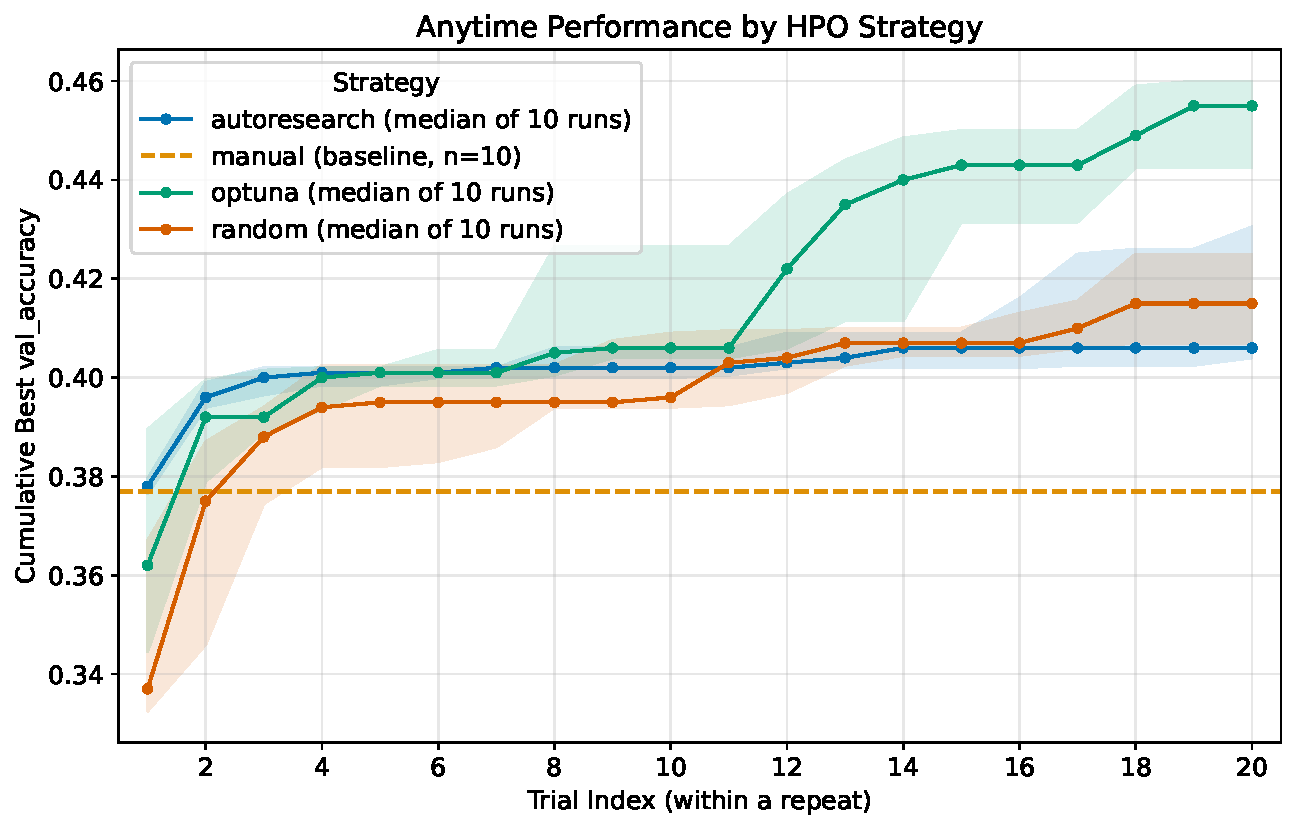
\includegraphics[width=\linewidth]{figures/phase3_anytime.pdf}
\caption{Anytime performance of the four strategies: median and IQR of
cumulative best \texttt{val\_accuracy} as trials progress, over 10 independent
repeats.}
\label{fig:anytime}
\end{figure}

\subsubsection{Search behaviour of the Autoresearch agent}
\label{sec:res-behaviour}

To identify the cause of the low variance, the number of unique hyperparameter
combinations proposed in each repeat was counted. Random Search and Optuna
produced 20.0 / 20 mutually distinct configurations in all 10 repeats (range
20--20), whereas Autoresearch attempted only 12.5 / 20 unique configurations on
average (range 10--17). Roughly 37\% of the search budget was thus consumed
re-running configurations already tried, and the phenomenon was observed
consistently across all 10 repeats rather than being confined to particular ones.

The pattern emerges more clearly in individual repeats. In repeat 8, the agent
explored by varying rank $16 \rightarrow 64 \rightarrow 32 \rightarrow 8
\rightarrow 32 \rightarrow 64$ over the first six trials, then became fixed after
the seventh trial on the combination \texttt{rank=64, alpha=256, lr=2.0e-4,
batch=2, targets=full}, proposing it 11 times consecutively. Notably,
\texttt{val\_accuracy} fluctuated between 0.388 and 0.444 while the identical
configuration was being re-run; this variation reflects the stochastic behaviour
of training and evaluation rather than any difference in configuration,
suggesting that the agent may have interpreted this noise as a performance
signal. In that repeat the agent broke out of the fixation by changing
\texttt{batch\_size} to 4 only on the final trial, and that configuration
recorded the repeat's best performance (0.4640).

The low performance of Autoresearch thus appears to stem not from poor quality of
the configurations it proposes --- its trial-level mean is in fact the highest ---
but from a reduced effective search budget caused by repeatedly proposing
identical configurations. This is, however, a post-hoc observation of result logs
and does not directly verify the agent's internal reasoning. The original
rationale texts are reproduced in Appendix~\ref{app:rationale}.

\subsubsection{Re-experiment with configuration consistency restored}
\label{sec:res-v2}

The account above attributes the low performance of Autoresearch to a reduced
effective search budget caused by duplicate proposals, and we argue in
Section~\ref{sec:discussion} that those duplicates may have originated not in
agent misjudgement but in configuration inconsistencies between the prompt and
the implementation. If that diagnosis is correct, removing the inconsistencies
should restore search diversity. The original condition was left untouched to
preserve reproducibility of the first run, and a separate condition,
\texttt{autoresearch\_v2}, was added with the configuration corrected. The search
space, model, dataset, \texttt{max\_steps}~$=200$, and repetition count are all
identical to the original; the changes are: (1) removal of the invalid parameter
\texttt{epochs} from the search space, whose proposed value the implementation
discarded; (2) a search-phase schedule expressed in budget proportions rather
than absolute trial numbers; (3) permission for rationale generation, lifting the
original ``JSON only'' constraint; (4) an explicit statement in the prompt of the
prohibition on duplicate proposals, which the code enforced but the prompt never
mentioned; and (5) injection of the actual budget (\texttt{total\_trials=20}) at
the call site, the default of 40 having truncated both the temperature and the
phase schedule at their midpoints.

\begin{table}[t]
\centering
\caption{The configuration-consistency re-experiment. Upper panel: diagnostic
metrics measured from the execution logs. Lower panel: pairwise Mann--Whitney $U$
tests at the run level. Rationale presence was determined by whether the raw
agent response consists solely of a JSON object; applying this criterion to the
original condition reproduces exactly the 147 JSON-only responses (73.5\%)
reported for that condition, so the two are compared under an identical
criterion.}
\label{tab:v2}
\small
\begin{tabular}{@{}lll@{}}
\toprule
Metric & Original Autoresearch & Autoresearch-v2 \\
\midrule
Unique configurations per repetition & 12.5 / 20 (10--17) & 18.90 / 20 (16--20) \\
Lowest temperature reached & 0.66 (planned floor 0.3) & 0.30 (as planned) \\
\texttt{exploitation} phase calls & 0 (expl.\ 166 / trans.\ 266) & 103 (expl.\ 51 / trans.\ 122) \\
Responses with a natural-language rationale & 53 / 200 (26.5\%) & 200 / 200 (100\%) \\
\midrule
Comparison (reference vs.\ target) & \multicolumn{2}{l}{$U$ \quad $p$ \quad rank-biserial $r$ \quad Verdict} \\
\midrule
Autoresearch (original) vs.\ Optuna & \multicolumn{2}{l}{16.00 \quad .0112 \quad $-0.68$ \quad Significant (Optuna superior)} \\
Autoresearch-v2 vs.\ Optuna & \multicolumn{2}{l}{31.50 \quad .1726 \quad $-0.37$ \quad Not significant} \\
Autoresearch-v2 vs.\ Autoresearch (original) & \multicolumn{2}{l}{66.00 \quad .2387 \quad $+0.32$ \quad Not significant} \\
\bottomrule
\end{tabular}
\end{table}

The intervention worked as intended (Table~\ref{tab:v2}). Unique configurations
rose from 12.5 to 18.90, approaching the 20.0 of Random and Optuna: the duplicate
proposals were a product of configuration inconsistency, not an intrinsic
limitation of the agent. Lifting the ``JSON only'' constraint also caused every
response to carry a natural-language rationale (200/200, mean length 620
characters), so the second requirement of RQ3 --- the provision of an
interpretable search rationale --- is confirmed at least as to whether rationales
are produced at all. What this establishes stops at the fact that rationales
\emph{were} produced; whether they correspond causally to the actual proposals, or
meet a quality an expert would accept as grounds for a decision, requires a
separate evaluation design that this study did not undertake. The
Kruskal--Wallis test across all five conditions gives $H = 29.72$, $p < .001$
($H = 27.92$ for the four-strategy set).

The run-level results point in two directions, and citing only one of them
distorts the finding. First, the significant deficit the original showed against
Optuna was eliminated: the original fell significantly short at $p = .0112$,
$r = -0.68$, whereas v2 is not significant at $p = .1726$, $r = -0.37$. The
confidence intervals agree --- the original's upper bound (0.4328) failed to
reach Optuna's lower bound (0.4368), leaving the intervals disjoint, whereas v2's
upper bound (0.4478) exceeds Optuna's lower bound, so the intervals overlap.
Moreover, v2's best single result of 0.4780 (repetition 9, trial 1030: rank 64,
alpha 256, lr 2.5e-4, batch 4, grad\_accum 16, targets full; closed 0.8156 / open
0.1562) is the highest value across all five conditions, surpassing Optuna's best
(0.4700).

Second, it nevertheless was not established that v2 outperforms the original
($p = .2387$). The effect size $r = +0.32$ is consistent with the direction of
improvement but does not reach significance at $n = 10$. What the re-experiment
demonstrates is therefore not that v2 is better than the original but that there
is no longer a basis for saying it falls significantly short of Optuna.

Third, restoring diversity did not translate directly into higher performance.
Although unique configurations rose 51\%, from 12.5 to 18.90, the run-level mean
improved only from 0.4184 to 0.4292. The per-repetition distribution shows why:
of the ten repetitions only two exceeded 0.42 --- repetition 2 (0.4303) and
repetition 9 (0.4230) --- while the remaining eight cluster in 0.39--0.41, and
the standard deviation of those two repetitions (0.034--0.040) is more than
double that of the rest (0.012--0.018). Securing search diversity increased the
opportunity to reach a high-performing configuration but did not reliably
guarantee reaching one. This is the structure behind v2 holding the single best
result across all conditions while its run-level mean still trails Optuna.

Fourth, the upper bound of the IQR for the trial at which the best result is
reached still touches the budget limit of 20 in v2 as well (median 15.0, IQR
[11.0, 20.0]). Even after configuration consistency is restored, a budget of 20
trials remains insufficient for this strategy.

We also record an operational failure. In the \texttt{autoresearch\_v2} execution,
8 of 200 trials failed before training began. The cause lay neither in the
hyperparameters nor in the training code but in a 120-second timeout that
occurred while the fine-tuning library transmitted execution-environment
statistics to an external hub immediately before training; the required model
weights were already in the local cache, so this call is unrelated to training.
After disabling that telemetry the 8 trials were re-run under identical
conditions and all completed normally, and the final aggregation is based on the
200 completed trials. The re-run trials received exactly the temperature and
phase schedule they would originally have been assigned, because the schedule is
computed from the count of completed trials, and the duplicate check consults the
full history, so these re-runs do not distort the unique-configuration metric or
the search trajectory.

\subsubsection{Summary of Phase 3}

The answer to RQ3 is negative. Under an identical search space and an identical
budget of 20 trials, the LLM agent's autonomous search fell significantly short of
Optuna (TPE) ($p = .0112$, $r = -0.68$) and was statistically indistinguishable
from random search (0.4184 vs.\ 0.4186). That all three automated strategies
exceeded the manual configuration nevertheless confirms both the validity of
automated search itself and the superiority of the established technique within
it. As the underlying cause we identify a reduced effective search budget caused
by duplicate proposals (12.5 of 20 unique configurations): an agent designed on
the premise of sequential self-improvement instead fell into early fixation, and
evidence was observed that it failed to distinguish the stochastic variation
appearing across re-runs of an identical configuration from a genuine improvement
signal.

The re-experiment confirmed this diagnosis. Removing the configuration
inconsistencies restored unique configurations from 12.5 to 18.90, so the
duplicate proposals were a product of the configuration rather than an intrinsic
limitation of the agent. The negative answer must therefore be read as applying
not to LLM agents in general but to an agent operated under this particular prompt
configuration. That qualification does not reverse the conclusion: even in the
corrected v2 condition the run-level mean reached only 0.4292, short of Optuna's
0.4490. What changed is that the deficit shrank to a level that is no longer
significant ($p = .0112 \rightarrow .1726$); that v2 is superior to the original
was not itself established in this sample ($p = .2387$). Restoring consistency
removed the grounds for asserting inferiority without creating grounds for
asserting superiority. The conclusion is limited to a single model
(Qwen3-VL-2B), a single dataset (PathVQA), a budget of 20 trials per strategy,
and the control condition \texttt{max\_steps}~$=200$; a substantial number of
Autoresearch runs were still improving when the budget was exhausted, and this
pattern persisted in v2, so results under a larger search budget could differ.

Cost must also be considered. Total training time for Autoresearch was 5,450
minutes, somewhat less than Optuna's 5,967 minutes, but Autoresearch incurs an
additional LLM API cost on every trial. Since it is a configuration that performs
worse while costing more, no grounds were found under these experimental
conditions for choosing Autoresearch over Optuna.
